\section{Classroom Study Settings}\label{classroom-study-settings}

\begin{figure}
\centering
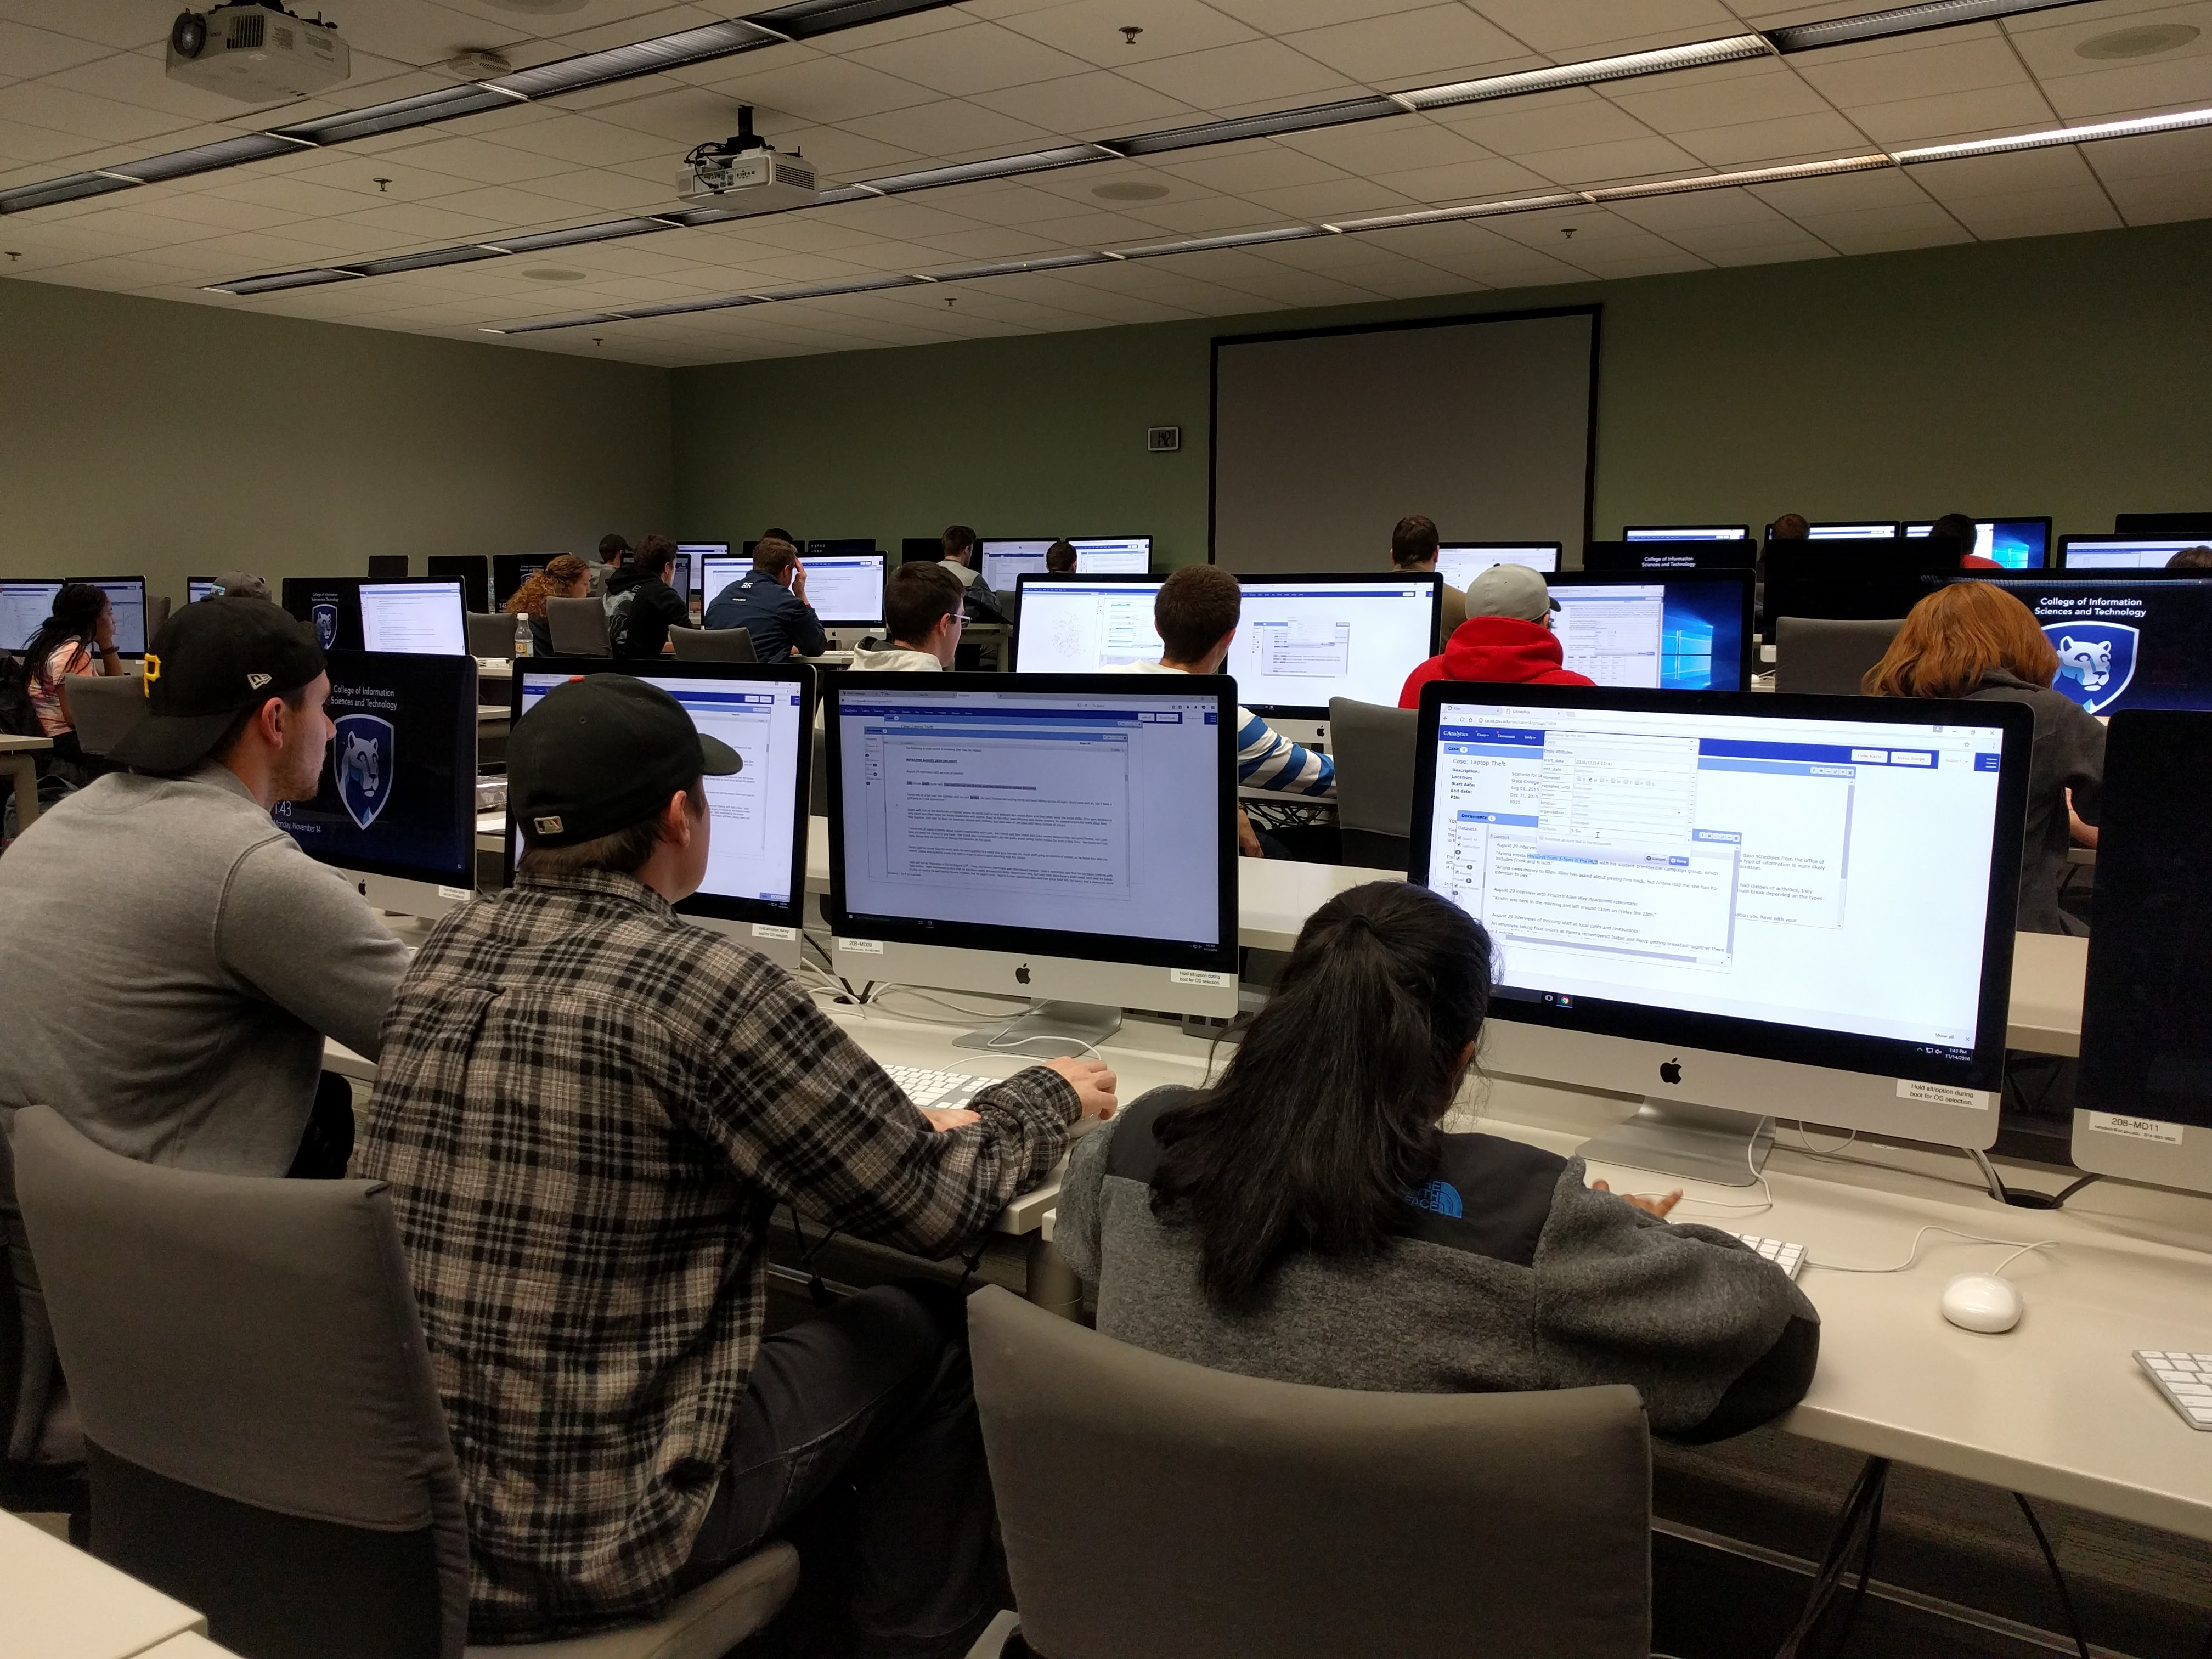
\includegraphics[height=1.5in]{./img/classroom_setting.jpg}
\caption{Classroom setting}\label{fig:classroom}
\end{figure}

The context for this study was an undergraduate course in an intelligence
training program in a US university (Figure~\ref{fig:classroom}). The program
was designed to train students to become professional intelligence analysts. A
key requirement of the course is to emphasize hands-on practice on team-based
intelligence analysis. During the first nine weeks, students learned strategic
knowledge (e.g.~bottom-up analysis and top-down analysis) and structured
analytic techniques, such as IEW, ACH and network analysis, and practiced to
apply these techniques to solving two small projects with state-of-the-art tools
including PARC ACH and IBM Analyst's Notebook.

Our study began from the 10th week of the course and lasted for one
week. The task was to investigate a series of bank robberies fabricated
by the course instructor. Teams were provided with a set of documents
pertaining to seven robberies, including police reports, witnesses
reports, video records, and news media. The task was designed
open-ended, which meant that there was no single answer to the task. The
instructor explained that the task was to simulate real world scenarios,
in which analysts always reasoned in the circumstances of uncertainty,
ambiguity, and complexity. The instructor told the students that 6 hours
was expected to complete the project, including in-class and
outside-class work. In the end of the project students were required to
submit a team report, describing their hypotheses, assumptions,
conclusions and supporting evidence.

Students were given a tutorial on CAnalytics a week before the project
began. One of the authors walked through features of CAnalytics and then
let students accomplish a small case analysis on their own pace. During
the study week, one author was always available to help with any
technical issues. Although students were encouraged to make full use of
CAnalytics, to ensure a naturalist environment students were always free
to employ any other tools that they believed useful.

Of the 98 students enrolled in the course (from two sections), 73
consented to participate in the study. Students were randomly assigned
into 25 teams (23 three-person teams and 2 two-person teams). Research
suggested that group size be an important factor in group collaboration,
thus two-person teams might behave differently from three-person teams.
We thus excluded data from the two-person teams in our analysis in this
paper. Also, from the log (and confirmed by their questionnaire), we
found that one team made little use of CAnalytics and opted for other
tools (Google Doc). Hence their data was also excluded. Thus in this
paper we reported the result from 22 teams.

All the students held major in the program of Security and Risk Analysis. Most
(75\%) of them were in the third academic year (3.05 years in average),
indicating that participants had been exposed to knowledge and techniques in the
domain of intelligence analysis. Participants' age ranged from 19 to 28 (20.3 in
average). 77\% of the participants were male.

We employed several data collection approaches. We administrated a
post-study questionnaire, which included questions using a seven point likert scale that measure individual's self-reported awareness (adapted from
\autocite{Convertino2011}), team communication (adapted from
\autocite{Convertino2011}), collective efficacy (adapted from
\autocite{Convertino2011}), perceived performance (adapted from
\autocite{Goyal2014}), and cognitive load \autocite{Hart1988}. The
questionnaire also included open-ended questions asking how the tool
helped or impeded their work. We captured user interactions with system
logs. Instead of simply logging low-level events like mouse click and
keyboard strokes, we recorded actions such as making an annotation and
deleting an entity. Finally, we reviewed team reports and graded them as
an indicator of team performance. We designed an assessment rubric
together with the course instructor. In analysis of the result, we
utilized artifact analysis, log analysis, and qualitative analysis of
the questionnaire.
